\selectlanguage{portuguese}
\section{Introducción}
\label{sec:introduccion}

A construção de uma linha de transporte de eletricidade requer
bastante preocupação. É muito importante construi-la de forma a
reduzir ao mínimo o risco de danificar pessoas. Tem que se assegurar
que a linha está a uma distância suficiente do solo e dos edifícios, e
que a construção é estável. Além disso, certos fatores devem ser
considerados, por exemplo a longitude do cabo elétrico produzido pelo
tempo, a temperatura do ambiente ou as velocidades máximas de ventos
que se registam e que possam produzir deterioração ou rotura do cabo.

%\begin{mybox} 
%  \vspace{-21pt}
\begin{figurebox}
  \vspace{20pt}
  \centering
  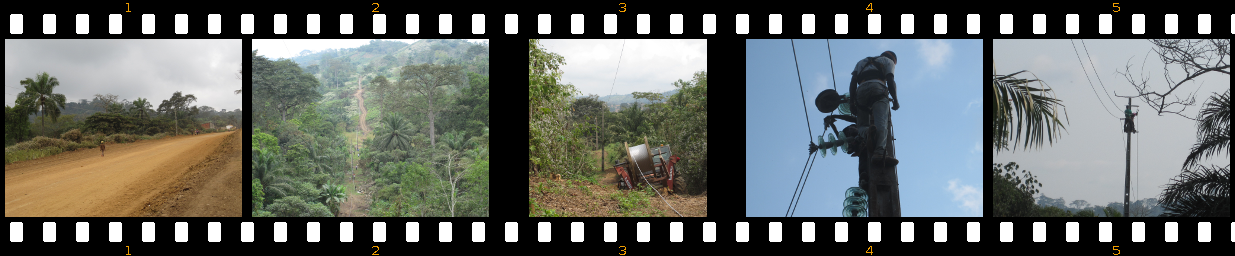
\includegraphics[scale=0.35]{InstalacionLinea.png}\\
  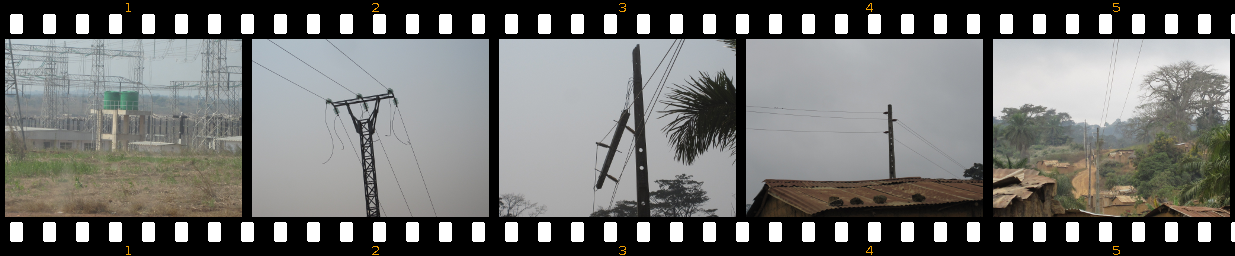
\includegraphics[scale=0.35]{InstalacionLinea2.png}\\
  Imagens de uma instalação elétrica em Angola\\ 
\end{figurebox}
% \vspace{-20pt}
%\end{mybox}

E eis onde a Matemática e a Física entram em ação. Com a sua ajuda
podemos construir uma linha elétrica que não só é segura, mas também
pode ser otimizado o valor do custo da construção. Anos de experiência
de engenheiros de todo o mundo mostram claramente que a matemática e a
física não se enganam, e existem diferentes modelos que cumprem
distintas normativas que garantem segurança. Em Angola existe um
regulamento de segurança de construção de linhas elétricas de alta
tensão e que pode encontrar no nosso formato online da revista no
separador de \emph{Documentação}, e será o que consideramos neste
artigo para realizar alguns cálculos mecânicos.

Na prática, existem diferentes softwares que permitem projetar as linhas elétricas e que têm as normativas do local específico onde se quer construir já pré-programadas. Mesmo quando existirem estes programas, o engenheiro que realiza o projeto com eles deve conhecer o funcionamento interno e ser capaz de interpretar os resultados do programa e ver se são consistentes. Ainda, o engenheiro deve ser consciente da normativa do local onde vai construir e ver as compatibilidades ou incompatibilidades da normativa que internamente tem o programa a utilizar.

Neste artigo vamos ver como a longitude do cabo elétrico de uma instalação elétrica varia pela tensão do seu próprio peso, pelo vento e pela temperatura atmosférica.


\section{O conceito seta da catenária}
\label{sec:parabola-vs-catenara}

No número de janeiro deste ano, estudámos em profundidade a curva da catenária e vimos que é a curva que descreve, por exemplo, um cabo elétrico suspenso em dois postes. Nesta secção vamos apresentar o que é a seta associada a uma catenária e apresentar as suas fórmulas. Este conceito é muito importante a ter em conta na construção de linhas energéticas e a chave para a segurança das pessoas.

\begin{wrapfigure}{r}{0.5\textwidth}
  \vspace{-.8cm}
  \begin{figurebox}
    \centering
    \begin{tikzpicture}
      \draw [bluesol] (0,0) -- (6,0);
      \draw [bluesol] (3,0) -- (3,5);
      \draw[domain=-3:3,smooth,variable=\x,redsol]
      plot({\x+3},{(exp(0.5*\x)+exp(-0.5*\x))});
      \draw[dashed] (0,2) -- (3,2);
      \draw[dashed] (0,0) -- (0,-1);
      \draw[dashed] (3,0) -- (3,-0.5);
      \draw[dashed] (6,0) -- (6,-1);
      \draw [<->,thick] (0,0) -- (0,2)
      node[midway,  rotate=90, yshift=-3mm] {{\tiny $a=\frac{T_v}{g\lambda}$}};

      \fill[bluesol] ( 0,4.7048) circle (0.1);
      \draw (-0.2,4.7048) node {$I$};

      \fill[bluesol] ( 6,4.7048) circle (0.1);
      \draw (6.3,4.7048) node {$S$};

      \draw[dashed] (0,4.7048) -- (6,4.7048);
      \draw [<->, thick,blue] (3,2) -- (3,4.7048)
      node[midway,  rotate=90, yshift=-3mm] {$f$ (setA)};
      \draw [<->, thick] (0,-0.5) -- (3,-0.5)
      node[midway, yshift=-2mm] {$v/2$};
      \draw [<->, thick] (0,-1) -- (6,-1)
      node[midway, yshift=-2mm] {$v$ (vão)};
      \draw [<->, thick] (6,0) -- (6,4.7048)
      node[midway,  rotate=90, yshift=-3mm]{$a\cosh(v/(2a))$};

      % \draw[red] (6,4.25) .. controls (5.833,2) .. (3,2);
      % \draw[<->]  (6,4) .. controls (5.8,3) and (4.1,1) .. (3,1);

    \end{tikzpicture}
    \caption{O gráfico da função $y =
      a\cosh(x/a)$.}
    \label{fig:1}
  \end{figurebox}
  \vspace{-.8cm}
\end{wrapfigure}

A seta de uma catenária é a máxima distância a partir da linha que conecta os pontos de suspensão do cabo para o cabo. Vamos dar forma matemática à seta associada à catenária. A fórmula geral da catenária é a seguinte:
\begin{equation}\label{cat:a}
  y = a\cosh\Big(\frac{x-C_1}{a}\Big)+C_2.
\end{equation}
Observe que as constantes $C_1$ e $C_2$ são constantes de translação no eixo $x$ e no eixo $y$ respetivamente, e por isso podemos considerar o caso quando $C_1 = C_2 = 0$. Assim, a Equação \ref{cat:a} reduzimo-lo à seguinte,
\begin{equation}\label{cat:b}
  y = a\cosh\Big(\frac{x}{a}\Big),
\end{equation}
que depende do parâmetro $a$ que é igual $\frac{T_0}{g\cdot\lambda}$ em que:
\begin{itemize}[noitemsep,nolistsep]
\item[$T_0$] é o valor da componente horizontal da tensão
(é constante em cada ponto do cabo, as suas unidades são Newtons [\si{N}]),
\item[$g$] é a aceleração devida à gravitação,
\item[$\lambda$] é o valor do peso do cabo dividido pela sua longitude.
\end{itemize}


\begin{wrapfigure}{r}{0.5\textwidth}
  \vspace{-2.1cm}
  \begin{mybox}
    \centering
    \emph{\textcolor{bluesol}{Séries de Taylor de cossenos e senos hiperbólicos.}}
    \begin{equation}
      \label{eq:10}
      \cosh(x)=1+\frac{x^2}{2!}+\frac{x^4}{4!}+\ldots,
    \end{equation}
    \begin{equation}
      \label{eq:11}
      \senh(x)=x+\frac{x^3}{3!}+\frac{x^5}{5!}+\ldots.
    \end{equation}
  \end{mybox}
  \vspace{-.8cm}
\end{wrapfigure}



%% Las unidades de la tensión son Newtons, pero en la práctica en
%% ingeniería es mucho más común utilizar kilogramos--fuerza, también
%% denominado \emph{kilopondio} ($[kgf]$).


Substituindo o valor de $a$, temos que a catenária se escreve como
\begin{equation}\label{cat:c}
  y = \frac{T_0}{g \lambda}\cosh \left(\frac{x\cdot g \lambda}{T_0} \right).
\end{equation}
% y si reescribimos por $T_v$ a la constante $\frac{T_0}{g}$ nos queda
% \begin{equation}\label{cat:d}
%   y = \frac{T_v}{\lambda}\cosh\Big(\frac{\lambda}{T_v}x \Big).
% \end{equation}


Vamos representar a equação da catenária escrita como na Equação (\ref{cat:c}) na Figura \ref{fig:1} a vermelho. Nesta figura podemos marcar em azul a distância seta e chamamos vão à distância entre os postes de fixação da catenária e que representamos com $v$. Deste modo, e observando o gráfico, é muito fácil dar fórmula à seta que denotaremos por $f$:
\begin{equation}
  \label{eq:4}
  f =  a\cosh\Big(\frac{v}{2a}\Big)-a=
  \frac{T_0}{g\lambda}\Big(\cosh\Big(\frac{g\lambda v}{2T_0}\Big)-1\Big).
\end{equation}
Se quisermos trabalhar com calculadora, podemos aproximar a seta por expressões polinómicas usando aproximações de Taylor (ver (\ref{eq:10})) de ordem quadrático por exemplo, da função cosseno hiperbólica. De este modo $f$ pode-se aproximar pela seguinte expressão:
 \begin{equation}
  \label{eq:12}
  f \approx{} \frac{v^2}{8a} = \frac{g\lambda v^2}{8T_0}.
\end{equation}

Desta forma, conhecer a seta permite-nos ter distâncias seguras controladas. O problema coloca-se quando introduzimos alterações de temperatura, vento ou o aumento de elasticidade do cabo produzido pelo tempo. Nas próximas secções vamos ocupar-nos das modificações de longitude do cabo pelas anteriores razões, e que devem ser tidas em consideração na altura de realizar uma instalação elétrica segura.
Finalmente, nesta secção vamos calcular a longitude de um segmento de catenária medido do ponto mais baixo para o ponto do lado da direita que corresponde à coordenada digamos $x$ e que denotamos por $l(x)$. Esta longitude pode ser calculada usando a fórmula que se demonstrou no artigo da catenária de janeiro deste ano dado pela Equação (3.3) ficando,
\begin{equation}
  \label{eq:3}
  l(x) = a\senh(x/a)=\frac{T_0}{g\cdot\lambda}\senh\Big(\frac{g\cdot\lambda}{T_0}x\Big).
\end{equation}
Outra vez, aproximando pela Série de Taylor (ver (\ref{eq:11})), temos que
\begin{equation}
  \label{eq:14}
  l(x) \approx{} x+\frac{x^3}{6a^2}=x+\frac{(g\cdot\lambda)^2}{6T_0^2}x^3.
\end{equation}
Portanto, a longitude do cabo é
\begin{equation}
  \label{eq:15}
  L = 2a\senh\Big(\frac{v}{2a}\Big)\approx{} v + \frac{v^3}{24a^2} = v
  + \frac{v^3(g\cdot\lambda)^2}{24T_0^2}.
\end{equation}

\section{Longitude do cabo pela tensão}
\label{sec:cable-y-la}

\begin{wrapfigure}{r}{0.5\textwidth}
  \vspace{-1.5cm}
  \begin{mybox}
    \centering
    \emph{\textcolor{bluesol}{Dados mecânicos do cabo LA-56}}
   \vspace{0.2cm}
   \begin{tabular}{llr}
     \toprule
     &Valor&Unidades\\
     \midrule
     Diâmetro & 9,5 & [\si{mm}]\\
      Peso & 0,189 & [\si{kgf}]\\
      Secção & 54,60 & [\si{mm^2}]\\
      Coeficiente de dilatação & 0,00001910 & \\
      Modulo elasticidade & 8100,00 & [\si{kgf/mm^2}]\\
      Carga rotura & 1670,00 & [\si{kgf}]\\
      \bottomrule
    \end{tabular}
  \end{mybox}
 \vspace{-1cm}
\end{wrapfigure}

Um problema que aparece quando se colocamos cabos elétricos, é que estes se prolongam se lhes for aplicada uma tensão. O parâmetro que corresponde à elongação do cabo é o módulo da elasticidade. Este parâmetro, por exemplo para um cabo tipo LA-56 é igual a 8100 quilogramas de força por um milímetro quadrado, isto é, que um metro de cabo prolonga-se  $1/(8100\cdot 54.6)\approx 0.002$ milímetros se aplicarmos um quilo de força (um quilo de força ´é igual aproximadamente a \SI{9.81}{N}). Na Tabela é apresentado um exemplo dos dados mecânicos do cabo tipo LA-56, que é um tipo de cabo que se usa comummente nas instalações elétricas. A fórmula do prolongamento unitário $\varepsilon$ é $\varepsilon=F/(A\cdot E)$,  em que $E$ é o módulo elasticidade também chamado o modulo de Young, $F$ a força, e $A$ a secção do cabo.

\begin{wrapfigure}{l}{0.5\textwidth}
  \vspace{-0.7cm}
  \begin{figurebox}
    \centering
    \begin{tikzpicture}
      \draw[->, very thick] (0,0) -- (6,0);
      \draw (3,-0.4) node {$T_0$};
      \draw [->, very thick] (0,0) -- (0,2);
    \draw (-0.4,1) node {$F_x$};
    \draw [->, very thick, bluesol] (0,0) -- (6,2);
    \draw [bluesol] (4.5,0.8) node {$T_x=\sqrt{T_0^2+F_x^2}$};
    \draw (0,-0.4) node {$P=(x,y)$};
    \draw [dotted, graysol] (0,2) -- (6,2);
    \draw [dotted, graysol] (6,0) -- (6,2);
    \draw [redsol, thick] (0,0) .. controls (2,0.8) and (2.5 , 1.2) .. (4,2.5);
    \draw [graysol, very  thick] (3,0) arc (0:18.435:3);
    \draw (2,0.3) node {$\alpha$};
      \draw [fill=black] (0,0) circle (0.1 );
    \end{tikzpicture}
    \caption{A tensão no ponto $x$}.
    \label{fig:5}
  \end{figurebox}
   \vspace{-0.5cm}
\end{wrapfigure}

Então, quando colocamos o cabo nos postes, este começa a sentir
tensão. Qual é esta tensão? Mostramos uma ilustração desta tensão num
ponto $(x,y)$ do cabo na Figura~\ref{fig:5}. Esta tensão, que chamamos
$T_x$ está quantificada como se segue:
\begin{displaymath}
  T_x=\sqrt{T_0^2+F_x^2}
\end{displaymath}
e na prática pode-se aproximar simplesmente à sua componente horizontal $T_0$.

Desta forma, se supormos que temos um cabo tipo LA-56 que vamos
pendurar entre dois postes e a sua longitude antes de pendurar era $L$
e a tensão medida depois de pendurar for $T_1$, então a sua longitude
$L_1$ depois de pendurar o cabo é
\begin{displaymath}
  L_1 = L(1+\varepsilon)=L\left(1+\frac{T_1}{AE}\right),
\end{displaymath}
cujas unidades são \si{kgf\per mm^2}.
%  y si reescribimos $t_1=T_1/A$ la anterior fórmula se simplifica como sigue:
% \begin{displaymath}
%   L_1=L(1+t_1/E)\textrm{, donde }t_1=T_1/A.
% \end{displaymath}
Então, se depois, uma força exterior como o vento alterar a tensão de
cabo para $T_2$, a mudança de longitude pode ser expressa como se
segue
\begin{equation}
 \label{eq:20}
 L_2-L_1=L\frac{T_2-T_1}{A\cdot E}.
\end{equation}

\section{Longitude do cabo pela temperatura}

A temperatura atmosférica é uma outra condição climática que pode
modificar a longitude do cabo. Se o cabo na temperatura de
\SI{20}{\degreeCelsius} tiver uma longitude $L$, na temperatura
$\theta$ sua longitude denotada por $L_{\theta}$ é
\begin{displaymath}
  L_{\theta}=L\cdot\alpha\cdot\theta,
\end{displaymath}
em que $\alpha$ é coeficiente de dilatação. Então, a diferença de
longitude devido à mudança de temperatura entre uma temperatura
$\theta_1$ e $\theta_2$ é:
\begin{displaymath}
  L_{\theta_2}-L_{\theta_1} = L\cdot\alpha\cdot(\theta_2-\theta_1).
\end{displaymath}
Se acrescentarmos esta modificação de longitude de temperatura à
mudança pela tensão do cabo da Equação \eqref{eq:20} temos que,
\begin{displaymath}
  L_2-L_1 = L\cdot\alpha\cdot(\theta_2-\theta_1)-L\frac{T_2-T_1}{AE}.
\end{displaymath}
Utilizando \eqref{eq:15}  or outro lado obtemos que
\begin{equation}
  \label{eq:21}
  L_2-L_1=\frac{v^3g^2}{24}\Big(\frac{\lambda_2^2}{T_2^2}-\frac{\lambda_1^2}{T_1^2}\Big).
\end{equation}
Então,
\begin{displaymath}
  L\cdot\alpha\cdot(\theta_2-\theta_1)-L\frac{T_2-T_1}{AE}=\frac{v^3g^2}{24}\Big(\frac{\lambda_2^2}{T_2^2}-\frac{\lambda_1^2}{T_1^2}\Big),
\end{displaymath}
e se supomos que $L\approx{}v$  então temos
\begin{equation}
  \label{eq:7}
  \alpha(\theta_2-\theta_1)-\frac{T_2-T_1}{AE}
  =\frac{v^2g^2}{24}\Big(\frac{\lambda_2^2}{T_2^2}-\frac{\lambda_1^2}{T_1^2}\Big).
\end{equation}

Um forte vento pode causar rotura do cabo. Por isso, no cálculo
mecânico de uma linha elétrica tem que se considerar este fator e
podemos ver isto refletido no ``Regulamento de segurança de linhas
eléctricas de alta tensão'' que impõe as condições que a linha tem 
que aguentar. Por exemplo, vamos ver os dois seguintes fragmentos de dois 
artigos:\\
{\bf Artigo 20º Hipóteses de cálculo:} ``Os condutores nus das linhas
devem ser calculados para a mais desfavorável das hipóteses
seguintes:''
\begin{itemize}[noitemsep,nolistsep]
\item[a)] na Zona Litoral Norte:
  \begin{itemize}[noitemsep,nolistsep]
  \item Temperatura de + 25° C e vento máximo habitual;
  \item Temperatura de +10° C e vento reduzido; 
  \end{itemize}
\item[b)] na Zona Litoral Sul:
  \begin{itemize}[noitemsep,nolistsep]
  \item Temperatura de + 25° C e vento máximo habitual;
  \item Temperatura de +5° C e vento reduzido; 
  \end{itemize}
\item[c)] na Zona Interior:
  \begin{itemize}[noitemsep,nolistsep]
  \item Temperatura de + 20° C e vento máximo habitual;
  \item Temperatura de 0° C e vento reduzido; 
  \end{itemize}
\end{itemize}
{\bf Artigo 23º Tensões máximas de tracção:} ``As tensões máximas de
tracção admissíveis para os condutores nus e para os tensores das
linhas não devem, para a hipótese de cálculo mais desfavorável
considerada no artigo 20º, ser superiores ao quociente das suas
tensões de rotura por 2,5.''


Em outros países, como por exemplo Estados Unidos ou Espanha, existe um outro fator que se deve considerar como o gelo, que durante o inverno se acumula acima do cabo. Mas este tipo de situação não se verifica habitualmente em Angola, e não a estudamos neste artigo.
\section{Sobrecarga de vento}
\begin{wrapfigure}{r}{0.5\textwidth}
  \vspace{-1.2cm}
  \begin{figurebox}
    \centering
    \begin{tikzpicture}
      \draw [dashed] (0,0) -- (6,0);
      \draw [dashed] (6,2) -- (6,0);
      \draw [<-, thick] (0,0) -- (0,2)
      node[midway,  rotate=90, yshift=-3mm] {$F_1$};
      \draw [->, thick] (0,2) -- (6,0)
      node[midway,  rotate=342, yshift=3mm] {$F'=\sqrt{F_1^2+F_2^2}$};
      \draw [->, thick] (0,2) -- (6,2)
      node[midway,  yshift=3mm] {$F_2$};

      \fill[bluesol] ( 0,2) circle (0.1);
      \draw (-0.2,2) node {$I$};



      % \draw[red] (6,4.25) .. controls (5.833,2) .. (3,2);
      % \draw[<->]  (6,4) .. controls (5.8,3) and (4.1,1) .. (3,1);

    \end{tikzpicture}\\
    \caption{Peso aparente do cabo com sobrecarga de vento.}
    \label{fig:2}
  \end{figurebox}
  \vspace{-.8cm}
\end{wrapfigure}

Agora vamos estudar como o vento influi na tensão do cabo. O regulamento considera que o vento atua na direção horizontal. Então se $F_1$ for a força devida ao peso do cabo e $F_2$ for a força do vento, a força total $F'$' é
\begin{equation}
  \label{eq:2}
  F'=\sqrt{F_1^2+F_2^2}.
\end{equation}


Mas, como podemos saber qual é a força máxima do vento? Isso está explicitamente indicado no regulamento no seguinte artigo:\\
{\bf Artigo 13º Pressão
  dinâmica do vento:} ``Os valores da pressão dinâmica do vento, em função da altura acima
do solo a que se encontra o elemento da linha sobre o qual se pretende
calcular a acção do vento, devem ser, para os escalões de altura que
se consideram, os indicados no quadro seguinte:''

\begin{table}[!h]
  \centering
  \begin{tabular}{ccc}
    \toprule
    Altura acima do solo [\si{m}] & 
    \multicolumn{2}{c}{Pressão dinâmica, $q$ [\si{Pa}]}\\
    \cmidrule(r){2-3}
    & Vento máximo habitual & Vento reduzido\\
    \midrule
    Até \SI{30}{m} & 750 & 300\\
    De \SI{30}{m} a \SI{50}{m} &  900 & 360\\
    Acima de \SI{50}{m} & 1050 & 420\\
    \bottomrule
  \end{tabular}
  \caption{Artigo 13º Pressão dinâmica do vento}
  \label{tab:3}
\end{table}

Os valores da pressão estão estimados utilizando medidas de velocidade do vento: regulamento.
``Os valores da pressão dinâmica do vento, constantes do quadro
anterior, foram calculados pela expressão:
\begin{equation}
  \label{eq:6}
  q = \frac{v^2}{16}9,81
\end{equation}
em que $v$, em metros por segundo, é a velocidade do vento,
considerada para os diferentes escalões de altura acima do solo.''

Desta forma, a Tabela~\ref{tab:3} apresenta a parte relevante do regulamento que indica os valores da pressão dinâmica do vento. Conhecendo o valor da pressão, podemos calcular a força utilizando a seguinte fórmula do {\bf Artigo 10º Ação do vento} do regulamento. ``No cálculo das linhas aéreas,
o vento deve considerar-se actuando numa direcção horizontal e a força
proveniente da sua acção considerar-se-á paralela àquela direcção,
determinada pela expressão:''
\begin{equation}
  \label{eq:5}
  F = \alpha c q S, \textrm{ em que:}
\end{equation} 
\begin{itemize}[noitemsep,nolistsep]
\item[$F$] em newtons [\si{N}], é a força proveniente da acção do vento;
\item[$\alpha$] é o coeficiente de redução;
\item[$c$] é o coeficiente de forma;
\item[$q$] em pascals [\si{Pa}], é a pressão dinâmica do vento;
\item[$S$] em metros quadrados, é a área da superfície batida pelo vento.
\end{itemize}



O {\bf Artigo 14º Coeficiente de redução} indica o seguinte:
``Os valores do coeficiente de redução a usar nos cálculos da acção do vento devem ser os seguintes:
\begin{itemize}[noitemsep,nolistsep]
\item[a)] 0,6, nos condutores e nos cabos de guarda; 
\item[b)] 1, nos apoios, nas travessas e nos isoladores.''
\end{itemize}
  
Además, {\bf Artigo 15º Coeficiente de forma}:

``Os valores dos coeficientes de forma a usar nos cálculos da acção do
vento devem ser os seguintes:''
\begin{itemize}[noitemsep,nolistsep]
\item[a)]  para condutores , cabos de guarda e isoladores:
  \begin{table}[!h]
    \centering
    \begin{tabular}{ccc}
      \toprule
      & Diâmetro do & Coeficiente de \\
      &  condutor [\si{mm}] & forma $c$ \\
      \midrule
      Condutores nus e cabos de guarda & Até 12,5 & 1,2\\
      & Acima de 12,5 e até 15,8 & 1,1\\
      & Acima de 15,8 & 1,0\\
      \midrule
      Cabos isolados em torçada & & Até 12,5\\
      Cabos auto-suportados e cabos tipo 8 && 1,8\\
      Isoladores && 1,0\\
      \bottomrule
    \end{tabular}
  \end{table}
\end{itemize}


Equipado com estas informações e fórmulas apresentadas, estamos em posição de calcular as setas e tensões máximas que pode ter uma catenária, e portanto ter as medidas de segurança controladas na construção de uma linha energética.


\section*{Anexo: Lei de Elasticidade de Hook}
Esta lei diz que o prolongamento  $\delta$ que experimenta um material elástico é proporcional à força $F$ aplicada ao material. Isto é
\begin{equation}
 \label{eq:1}
 F = k \cdot \delta.
\end{equation}
em que $k$ é uma constante chamada a constante de rigidez com unidades com
unidades $[N/m]$.

A forma mais comum de representar esta lei para um material elástico como um cabo ou uma corda é utilizando o módulo de Young. Nesta representação é considerado o prolongamento unitário, isto é
\begin{displaymath}
 \varepsilon = \frac{\delta}{L},
\end{displaymath}
em que $L$ é a longitude do cabo antes do prolongamento. Então \eqref{eq:1} podemos reescrever como
\begin{displaymath}
 \varepsilon = \frac{F}{kL}.
\end{displaymath}
É bastante claro, que se um cabo for duas vezes mais grosso, a força tem que ser dupla. Por isso, é introduzido um parâmetro de um material que é independente da secção transversal do cabo. Por isso, reescrevemos esta equação como
\begin{displaymath}
 \varepsilon = \frac{F/A}{kL/A}=\frac{F}{AE}.
\end{displaymath}
em que $E=kL/A$ é o módulo de Young e as suas unidades são então
$[N/m^2]$ ou equivalente $[kg/(s^2m)]$. Isto também se pode simplesmente denotar $[Pa]$. 

%%% Local Variables: 
%%% mode: latex
%%% TeX-master: "matematicaseningenieria"
%%% End: 


